\documentclass[12pt]{article}
\usepackage[utf8]{inputenc}
\usepackage[T1]{fontenc}
\usepackage{titlesec}
\usepackage{enumitem}
\usepackage[left=2.54cm,top=3cm,right=2.54cm,bottom=3cm]{geometry}
\usepackage[]{csquotes}
\usepackage[sorting=none]{biblatex}
\usepackage{hyperref}
\usepackage{graphicx}
\usepackage{upgreek}
\usepackage{setspace}
\usepackage{longtable}
\usepackage{eurosym}
\usepackage{rotating}
\usepackage[table]{xcolor}
\usepackage[acronym,toc]{glossaries}

\renewcommand{\arraystretch}{1.3}
\renewcommand{\glsnamefont}[1]{\textbf{#1}}

\graphicspath{ {00Images/} }
\DeclareGraphicsExtensions{.png,.pdf}
% \DeclareGraphicsExtensions{.pdf,.png} % - CHANGE TO THIS

\addbibresource{mendeley.bib}
\setlength{\parindent}{1cm}

% Acronyms %%%%%%%%
\makeglossaries

% \newacronym{}{}{}
% \newacronym{}{}{}
% \newacronym{}{}{}
% \newacronym{}{}{}


%%%%%%%%%%%%%%%%%%% 

\begin{document}
% 
\tableofcontents
\pagebreak

\begin{singlespacing}
\setglossarystyle{long}
\printglossary[type=\acronymtype, title=List of acronyms and abbreviations, toctitle=List of acronyms and abbreviations, nonumberlist]
\printglossary
\end{singlespacing}

\section{Introduction}
% 
Exchanging cryptocurrencies is becoming a regular task for an increasing number of people. There are countless different platforms that offer this service, ranging from simple wallets that offer currency exchange as additional service, to massive trading platforms with daily market cap of millions of dollars. All of these exchanges, however share one common feature - when making a transaction, we need to trust them with our funds. Let us consider an imaginary cryptocurrency exchange website \textit{Exchange.net}. This website offers exchange from Bitcoin to Litecoin and vice versa. Whenever we wish to use Exchange.net, we need to transfer our funds to the company's account, exchange the funds on the website and then withdraw our exchanged funds again. Until we make the withdrawal, Exchange.net has full control over our money. If the company suddenly goes out of business, or gets attacked, we may never get our funds back! There have been various cases, where deposited funds were lost or stolen, with the most famous case of the Japanese-based Bitcoin exchange Mt. Gox, where USD 380 million worth of Bitcoins were stolen in 2014~\cite{Popper2014ApparentTimes}.

There are numerous reasons to buy cryptocurrency, ranging from a value holding purposes to short-term trading. However, the trust in the cryptocurrency is somewhat unavoidable. Regardless of our motivation, whenever we acquire a (crypto-) currency, we believe that it will retain value at least until we exchange it for other services or goods. Researchers and developers have been trying to create a cryptocurrency for a long time. As early as 1983 anonymous digital money was proposed by an American cryptographer David Chaum~\cite{Chaum1983BlindPayments}. 

Today's cryptocurrencies, such as Bitcoin and Litecoin are thus only the continuation of a long lasting effort to develop a currency with sufficient guarantees against misuse, such as double-spending or theft. The wide-spread adoption of these currencies indicates, that the guarantees against misuse are indeed sufficient -- in other words, that the users trust the cryptocurrency. If this was not the case, it probably would not be used. On the other hand, the trust in the exchange platform is more questionable. Some advise not to store any funds in the exchange for longer periods of time and to make deposits to a secured wallet right away - because it is believed the funds are more vulnerable in an exchange~\cite{McIntosh2018HowScams}.

In this project we address this problem and propose a system, where the trust in the currency is used for making the exchange process of exchange safer. To accomplish this task, we have used the Ethereum system, which is the second most popular cryptocurrency as of today. Ethereum gives the possibility of running \emph{smart contracts} -- small programs that are run by many computers around the world at the same time. This provides assurance, that no-one will tamper with the code and that no-one can manipulate with the outcome of a smart contract. 
% 
\footnotetext{By market cap. \url{https://coinmarketcap.com/all/views/all/}, accessed 21-05-2018}
% 
In this project, we investigate, if smart contracts could be used to facilitate cryptocurrency exchange and how such system could operate. We implement a system, that uses an Android application to deploy smart contracts to the Ethereum network. These contracts are used to control the trading process and function. We demonstrate the operation of this prototype in a model scenario, where we transfer Bitcoin and Ether between two trading parties.

The rest of the report is structured as follows: we first define the problem in the \textit{\ref{sec:problem-formulation} Problem Formulation} chapter. Afterwards, we describe the methods and processes, used in this project in the \textit{\ref{sec:methodology} Methodology} chapter and introduce the basic concepts of cryptocurrency exchange in \textit{\ref{sec:background} Background}. Later, we investigate the existing systems that are relevant to our proposal in the \textit{\ref{sec:SOTA} State of the Art} chapter, before we describe considerations for the system architecture in the \textit{\ref{sec:system-design} System Design}. Finally, we elaborate on the requirements and system implementation details, together with a short evaluation and a model scenario in the \textit{\ref{sec:implementation} Implementation and Evaluation} chapter. The outcomes of this project are debated in \textit{\ref{sec:discussion} Discussion}, before the report is concluded in the \textit{\ref{sec:conclusion} Conclusion}. This report has 4 appendices.
\pagebreak
\section{Problem Formulation}
% 
Problem formulation, v0.1:

\begin{itemize}
    \item \textit{How to implement a crypto-currency exchange, using smart contracts?}
\end{itemize}
\pagebreak
\section{Background}\label{sec:background}
% 
In this section, we will explain some of the main concepts used in this project. This section is needed to establish a common understanding behind these topics, so that unambiguous discussion can follow.

First, we will briefly talk about the concept of currency and its exchange. Afterwards we will define what a cryptocurrency is and how it differs from a fiat currency. 
% 
\subsection{Fiat  currency}
% 
Currency, as the medium of exchange for goods and services, is the basis of trade. Since the history of humanity, we have always engaged in some sort of a trade. Whenever we needed a commodity we do not posses, we needed to get this commodity by trading it for something else. This exchange of commodities was referred to as barter trade. Barter trade, however was not always suitable, since it required the alignment of wants and was not very scalable for large transactions~\cite{Carroll2015CreatingExchange}. To overcome these limitations, money was invented. Money can be seen as opposition to barter trade. In the beginning, cattle, salt or precious metals were used as 'comodity money', later coins were invented. But money is not necessarily the same as `currency'.  Currency is more specific form of money. Currency, in traditional meaning is issued and controlled by the government\footnotemark.
% 
\footnotetext{\url{https://www.investopedia.com/terms/c/currency.asp}, accessed 22-03-2018}

Until 1971, every US dollar could be exchanged for its respective value in gold. This system is known as a ``representative currency'', since the entire currency is represented by the amount of gold the government posses. This is also called ``Gold standard'' and is currently rarely used. In opposition to representative currency stands the fiat currency. 

Fiat currency is a currency that is issued and controlled by the government and is declared a legal tender in respective country. However, unlike the representative currency, it is not backed by any physical commodity and its value is simply derived from the supply-demand relationship\footnotemark. Most of today's currencies, including US Dollars, Euros, Yens or Danish Crowns are fiat currencies.
% 
\footnotetext{\url{https://www.investopedia.com/terms/f/fiatmoney.asp}, accessed 22-03-2018}
% 
\subsection{Cryptocurrency}
% 
Merriam-Webster dictionary defines cryptocurrency as a \textit{``form of currency that only exists digitally, that usually has no central issuing or regulating authority, but instead uses a decentralised system to record transactions and manage the issuance of new units, and that relies on cryptography to prevent counterfeiting and fraudulent transactions''}\footnotemark.
% 
\footnotetext{\url{https://www.merriam-webster.com/dictionary/cryptocurrency}, accessed 27-03-2018}

Digital currency means that we can only access it in a digital world. This is opposed to fiat currencies, which have both physical representation of the currency (coins and notes) and digital representation (money in a bank). Technology of cryptography assures that the currency will only be used in the intended way. Fraud cases, such as producing additional fake currency, double spending, or unauthorised transfer need to be prevented. With the physical cash, measures can be taken to prevent tampering with the notes and coins, such as watermarks, special print or holograms. In the digital world, these measures need to be enforceable and verifiable by the computer.

There are numerous technical characteristics of cryptocurrencies. However, the most prominent ones, as listed by many research works~\cite{Lansky2018PossibleCryptocurrencies} are the following:
\begin{enumerate}[noitemsep]
    \item The system does not require a central authority, distributed entities achieve consensus on its state.
    \item The system keeps an overview of cryptocurrency units and their ownership.
    \item The system defines whether new cryptocurrency units can be created. If new cryptocurrency units can  be  created,  the  system  defines  the  circumstances  of  their  origin  and  how  to  determine  the ownership of these new units.
    \item Ownership of cryptocurrency units can be proved exclusively cryptographically.
    \item The system allows transactions to be performed in  which ownership of the cryptographic units is changed. A transaction statement can only be issued by an entity proving the current ownership of these units.
    \item If  two  different  instructions  for  changing  the  ownership  of the  same  cryptographic  units  are simultaneously entered, the system performs at most one of them.
\end{enumerate}

Public-key encryption and hashing are the two most used cryptographic concepts used in cryptocurrencies. In several cryptocurrencies, hashing is used to maintain a consensus over the network's state and public-key cryptography is used to prove the ownership of the cryptocurrency\footnotemark.
% 
\footnotetext{Not all currencies use the public-key cryptography. For example, Fawkescoin only uses hashing for both state consensus and currency ownership~\cite{Bonneau2014FawkescoinCryptography}}

\subsubsection{Motivation for cryptocurrencies}
Naturally, the cryptocurrency was not entering a blue ocean upon its inception. Today, all countries have a generally accepted currency, usually issued by central bank. This system, however, has certain limitations. The main drawback is virtually unlimited supply of the currency. A government can issue more money, as it deems necessary. As a consequence, the value of a fiat currency can therefore decrease drastically (e.g. the value of Zimbabwean dollar dropped by hundreds of percents in 2006~\cite{MichaelWines2006HowZimbabwe} or hyper-inflation case in Venezuela in 2018~\cite{ManuelRueda2018VenezuelasMoney}). Secondary, the government could use its ability to control the currency to influence anti-governmental organisations or groups by limiting their access to their funds. This can be a problem for whistle-blower organisations (such as WikiLeaks) or for freedom movements in repressive regimes.

Cryptocurrency overcomes these problems, since there is no central authority that could control the currency. Every user of the currency can participate in making the more secure by running specialised software on their computer. The issue of units of the currency is controlled by the system in a well-defined and expectable manner. The trust in the central bank is thus replaced by trust in the cryptocurrency. In the next section we will explore, how blockchain enables this decentralisation.
% 
\subsection{Blockchain}
% 
Since the inception of a digital currency Bitcoin (described in the following section) in 2009, blockchain has been part of the discussions about this novel approach to currency. Over the time, the perception shifted from seeing blockchain just as a part of cryptocurrency into seeing it as an separate, innovative, even disruptive technology. Some media mark \textit{blockchain} to be the word of the year 2017\footnotemark, while others comparable it to inception of the Web in 1990s \cite[p. 14]{Swan2015BlockchainEconomy}.
% 
\footnotetext{\url{https://www.theguardian.com/technology/2018/jan/30/blockchain-buzzword-hype-open-source-ledger-bitcoin}, accessed 28-03-2018}

From the perspective of cryptocurrency, blockchain is a public ledger, that contains all the transactions of the cryptocurrency to date \cite{Swan2015BlockchainEconomy}. It is distributed among all the computers participating in the consensus process. Since it contains all the past transactions (since the inception of the currency), data is never deleted from the blockchain. All changes happen only as amendments to the latest version of the blockchain.

A \textit{change} could be virtually any data. For example, it could be details of latest transactions (as is the case with Bitcoin) or newly deposited agreements (as in Quorum - enterprise level ledger \footnotemark ). This \textit{change} is called a \textit{block}. Blocks are the fundamental parts, that make up the blockchain. When a new blockchain is created, a first set of changes becomes the first block.
% 
\footnotetext{Quorum is a blockchain-based private storage for agreements. Its intended users are enterprises in the finance industry, who are trading financial derivatives and who need to reach an agreement, while maintaining acceptable level of privacy.
\begin{flushleft}
\url{http://fortune.com/2016/10/04/jp-morgan-chase-blockchain-ethereum-quorum/}, accessed 28-03-18
\url{https://www.jpmorgan.com/global/Quorum}, accessed 28-03-18
\end{flushleft}
}
% 
When more changes are made (for example, more transactions are processed), a new block is created. The creation of a new block involves computing a hash value of the previous block. This hash value is then included in the new block, together with the data comprising the change. By including the hash value of the old block in the new block, these two blocks are now linked. All the blocks in the blockchain are linked together in such fashion. Figure \ref{fig:blockch-basics} illustrates this principle. 
% 
\begin{figure}[h]
    \centering
    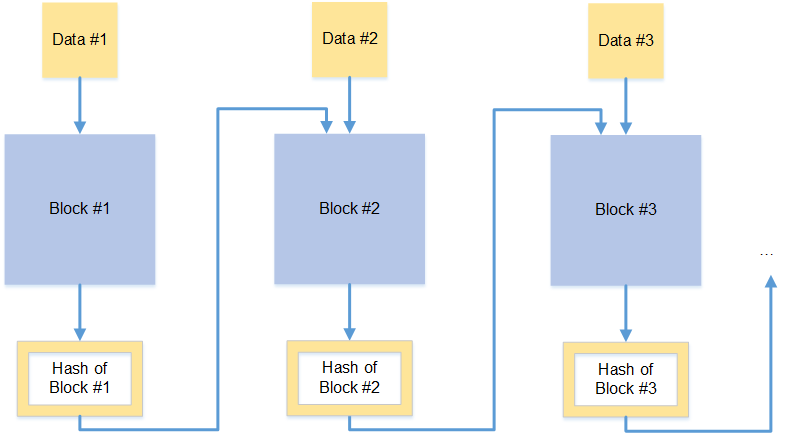
\includegraphics[width=.95\textwidth]{blockchain-basics}
    \caption{The basic architecture of a blockchain. If Block \#1 is the first block in the chain, it is also referred to as the \textit{genesis block}.}
    \label{fig:blockch-basics}
\end{figure}

It is not possible to alter the past blocks in the blockchain. In order to accomplish this, we would need to find such a combination of data, that would produce the same hash. This violates the pre-image resistance property of the hash function. Alternative technique could be to change the data in block \textit{n}, then calculate new hash and include it in block \textit{n+1} and so on, recalculating every subsequent block \cite[3]{NakamotoBitcoin:System}.

The decentralisation of the blockchain prevents this. Every participating node maintains and updates its own copy of the blockchain. When there is a dispute about the correct version of the blockchain, the version that is present on most nodes is chosen as the correct one and the other versions are discarded. Therefore, an attacker would need to control the majority of the nodes in the network in order to include counterfeit data in the blockchain.

Based on the use of the blockchain, we can distinguish between three `levels' \cite{Swan2015BlockchainEconomy}:
\begin{itemize}[noitemsep, nolistsep]
    \item \textit{Level 1} is blockchain used with currency only. The data here are transactions of that currency. Level 1 of blockchain would be for example Bitcoin.
    \item \textit{Level 2} includes smart contracts and more advanced transactions and agreements than Level 1. However, Level 2 of blockchain is still tied to financial applications in some way. Example of Level 2 blockchain is Ethereum platform.
    \item \textit{Level 3} of blockchain includes usage outside of financial applications, in sectors such as government or health-care \cite{Swan2015BlockchainEconomy}.
\end{itemize}

% Motivate problems with cryptocurrency? Double spending problem and byzantines general problem? 
% Central bank system - problems?
% Decentralised system - solutions
% mentioned briefly - drawbacks
% narrower definition of blockchain - list of transactions for a cryptocurrency
% broader definition - number of other applications, Blockchain 2.0 and Blockchain 3.0 as described by Swan
% 
\subsection{Bitcoin}
% 
Created in 2009, Bitcoin is the first ever digital currency, that operates without a central authority in a completely decentralised manner. It is a cryptocurrency with largest market capitalisation\footnotemark and probably the most famous cryptocurrency worldwide.
% 
\footnotetext{Over USD 115 billion as of 01-04-2018. \url{https://coinmarketcap.com/}, accessed 01-04-2018
}
% 
Bitcoin was proposed by a person or a group under the pseudonym Satoshi Nakamoto, whose identity is not known to date~\cite{Feins2017SatoshiBitcoin}. The initial proposal consisted of a white-paper describing the system~\cite{NakamotoBitcoin:System} and the reference implementation written in  C++ \footnotemark.
% 
\footnotetext{Original repository has been moved from SourceForge and can now be found on Github. \url{https://github.com/bitcoin/bitcoin/tree/4405b78d6059e536c36974088a8ed4d9f0f29898}, accessed 01-04-2018}

In the white-paper, Nakamoto proposes a decentralised currency, based on a proof-of-work blockchain. The blockchain is made up of blocks, where each block comprises a different set of transactions~\cite{Decker2013InformationNetwork, Judmayer2017BlocksMechanisms}.

\subsubsection{Proof of work}
To include a new block in the blockchain, certain amount of work needs to be carried out by the node. This is a protection against the attempts to include counterfeit data in the blockchain. As discussed earlier, to falsify a past block, an attacker would need to recalculate all the subsequent blocks. Furthermore, they would need to provide proof-of-work for all the subsequent blocks. Since the \acrfull{pow} is computationally intensive, it would be practically impossible for the attacker to outpace the honest nodes~\cite{NakamotoBitcoin:System}.

In case of Bitcoin, the proof-of-work consists of finding such a hash value, that is below a given constant -- \textit{target}. In Bitcoin, this hash value is computed over the hash value of previous block, timestamp\footnotemark, root hash of the transactions\footnote{Transactions are ordered in a Merkle tree.} and a random number, called \textit{nonce}. The work of the nodes consists of generating a new nonce and computing a new hash. If value of this hash is smaller than the target, a valid block is produced and can be broadcasted to the other nodes. Figure~\ref{fig:blocks-bitcoin} shows the composition of the block in detail. By design, a new block should be mined approximately every 10 minutes. The network automatically adjusts the value of the target to meet this requirement (if the value of the target remained the same, increasing speed of computers would result in faster block production speed over time)~\cite{Decker2013InformationNetwork}.
% 
\footnotetext{The timestamp is a local UNIX time of the node. However, this timestamp does not to be very accurate (approximate allowed accuracy is $\pm$ 1 hour). It can happen, that the timestamps in blocks are not in order. The goal of the timestamp is to increase the difficulty of forging the blocks. \url{https://en.bitcoin.it/wiki/Block_timestamp}, accessed 01-04-2018}
% 
\begin{figure}[ht]
    \centering
    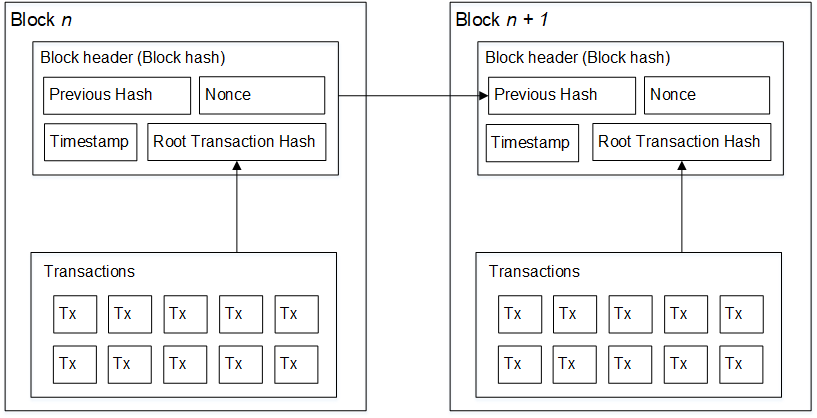
\includegraphics[width=.95\textwidth]{blocks-bitcoin}
    \caption{Composition of the Bitcoin blockchain. Work of a node consists of repeatedly hashing the block header, trying out different nonce every time.}
    \label{fig:blocks-bitcoin}
\end{figure}
% 
\subsubsection{Network of nodes}
Each node carries out work at its own pace, trying different values for nonce and hashing the block header. Essentially, this is simply trying using the brute force to produce a hash below a threshold. This process is also referred to as \textit{mining}. Once the hash is below the current threshold, a new block is mined. The new block is then broadcasted to all the nodes connected to the network~\cite{NakamotoBitcoin:System}. When a node receives a block it has not seen before, it first verifies the transactions in the block and then introduces it to its peers. The average time for a block to reach the whole network is 12.6 seconds~\cite{Decker2013InformationNetwork}. It is well below the block generation speed (1 block approximately every 10 minutes), however, it is not crucial for the network that every node has a copy of the latest block: ``\textit{If a node does not receive a block, it will request it when it receives the next block and realises it missed one.}''~\cite{NakamotoBitcoin:System}.
% 
\subsubsection{Transactions and accounts}
A Bitcoin transaction is the act of moving the funds from one account to another~\cite{Judmayer2017BlocksMechanisms}, as illustrated in Figure~\ref{fig:bitcoin-tx}. To explain this process, we must first define the notion of an account.

\begin{figure}[ht]
    \centering
    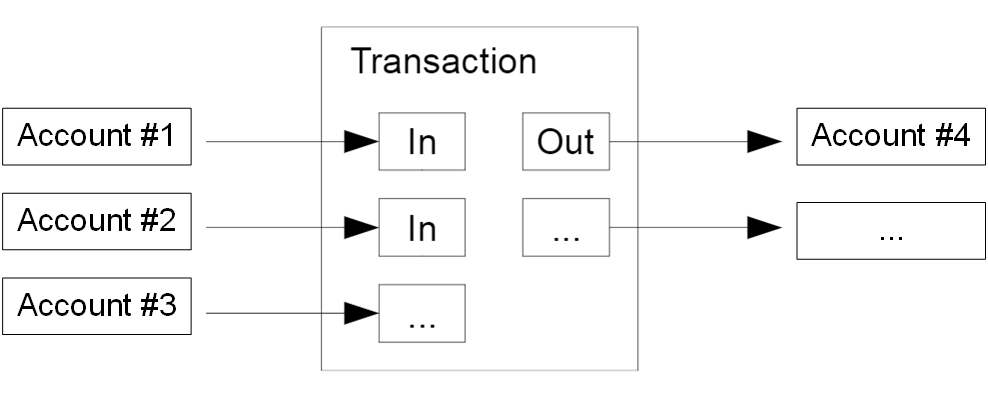
\includegraphics[width=\textwidth]{bitcoin-tx}
    \caption{A Bitcoin transaction representation. Each transaction has to have at least one input and one output. The inputs and outputs can have various values, but the total sum of the inputs needs to be equal to or greater than the number of outputs. The only exemption from this rule is the reward for the miner that found a new block. Such transaction only has outputs and no inputs. Taken from~\cite{NakamotoBitcoin:System}, edited.}
    \label{fig:bitcoin-tx}
\end{figure}

An account is a pair of a public and private key. Bitcoin uses the \acrfull{ecdsa} for the key pair generation~\cite{Decker2013InformationNetwork}. The account is identified by its public address, which is generated from the public key through a series of hashes. Figure~\ref{fig:public-address-gen} describes this process in further detail.
% 
\begin{figure}[p]
    \centering
    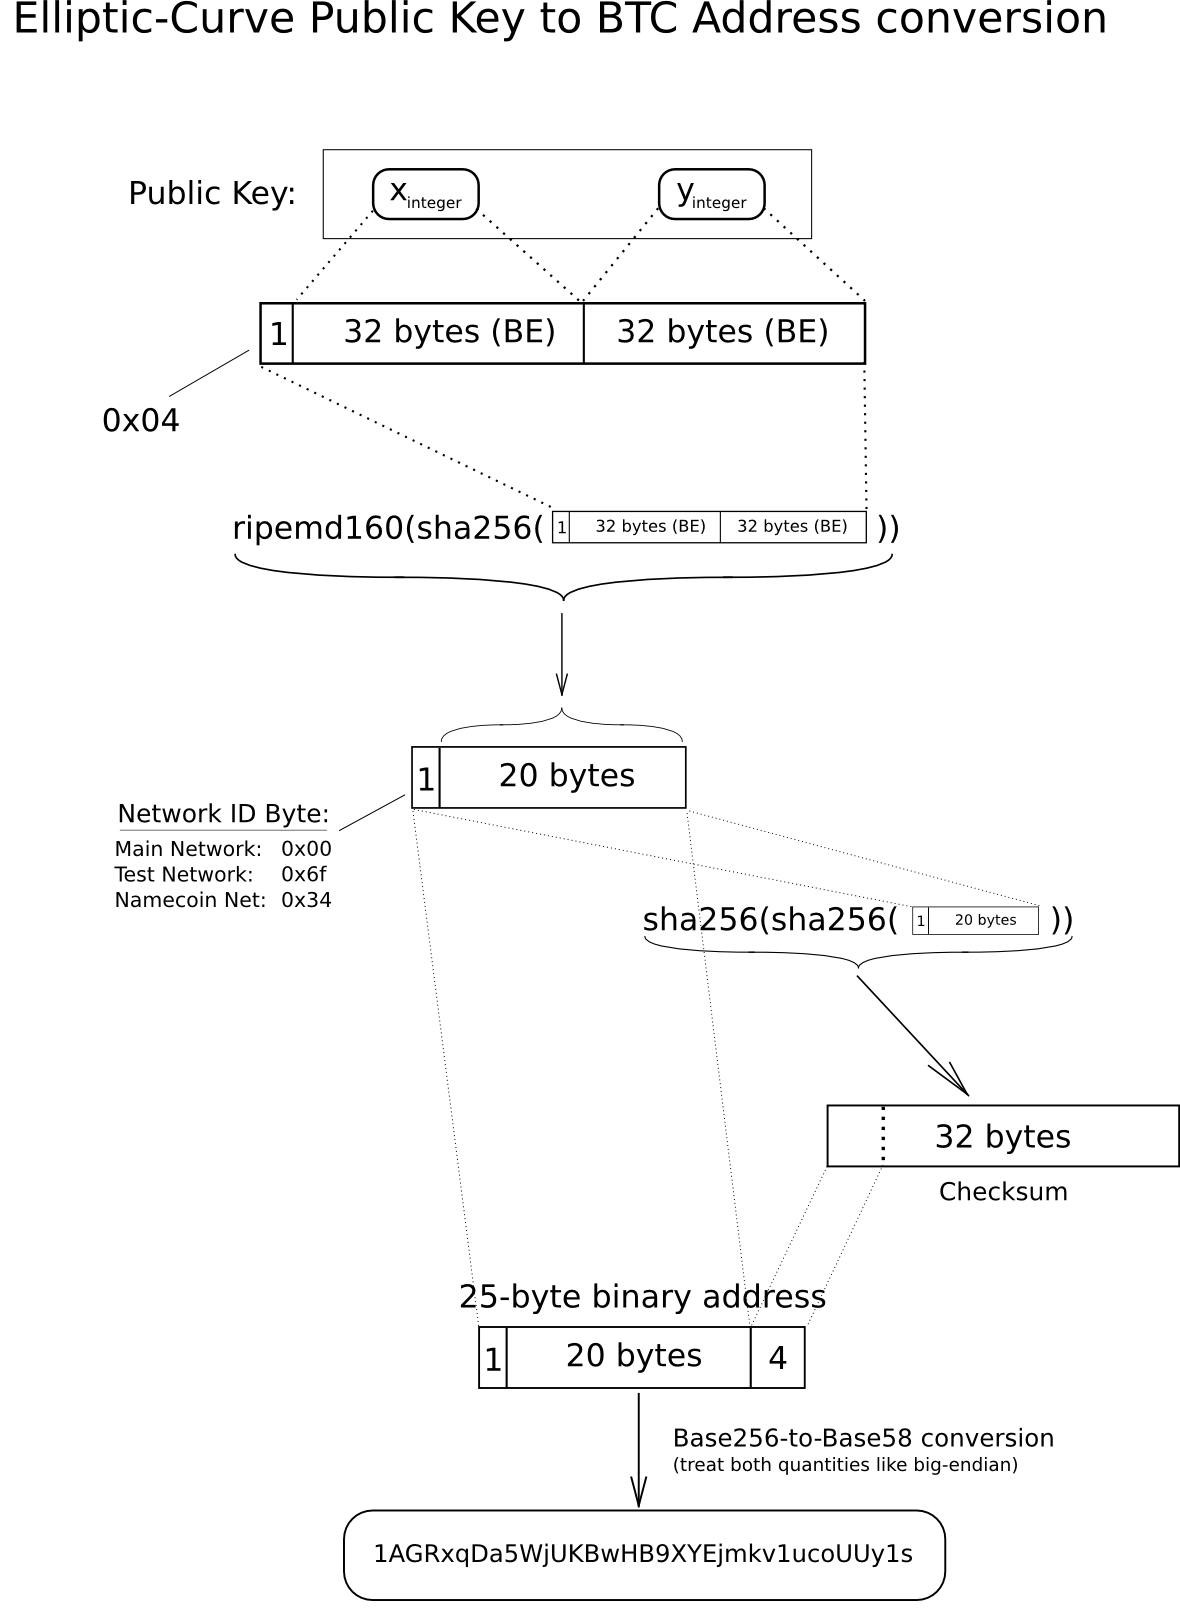
\includegraphics[height=.85\textheight]{PubKeyToAddr}
    \caption{First, a public key and a prefix are hashed using SHA-256 and then RIPEMD-160. This value is hashed twice with SHA-256 to generate a checksum. The result is composed of 1 network byte, RIPEMD-160 hash and first 4 bytes of checksum.}
    \label{fig:public-address-gen}
\end{figure}

A transaction contains a number of inputs and a number of outputs. The sum of inputs must be equal or greater than the sum of the outputs~\cite[p. 27]{Judmayer2017BlocksMechanisms}. In case the sum of the inputs of the transaction is greater than sum of the outputs, the excess is collected by the miner as the \textit{transaction fee}.

Every unit of the currency has a history of transactions up to its origin. This chain of ownership verifies the validity of that particular unit and serves as a proof, that the unit is not counterfeit. Transferring funds from one account to another comprises hashing the public address of the future owner and hash of the last transaction. The resulting hash is then singed with the private key of the previous owner~\cite{NakamotoBitcoin:System}, as illustrated in Figure~\ref{fig:chain-ownership}. Once the transaction is signed, it is distributed to the network and can be included in a block.
% 
\begin{figure}[ht]
    \centering
    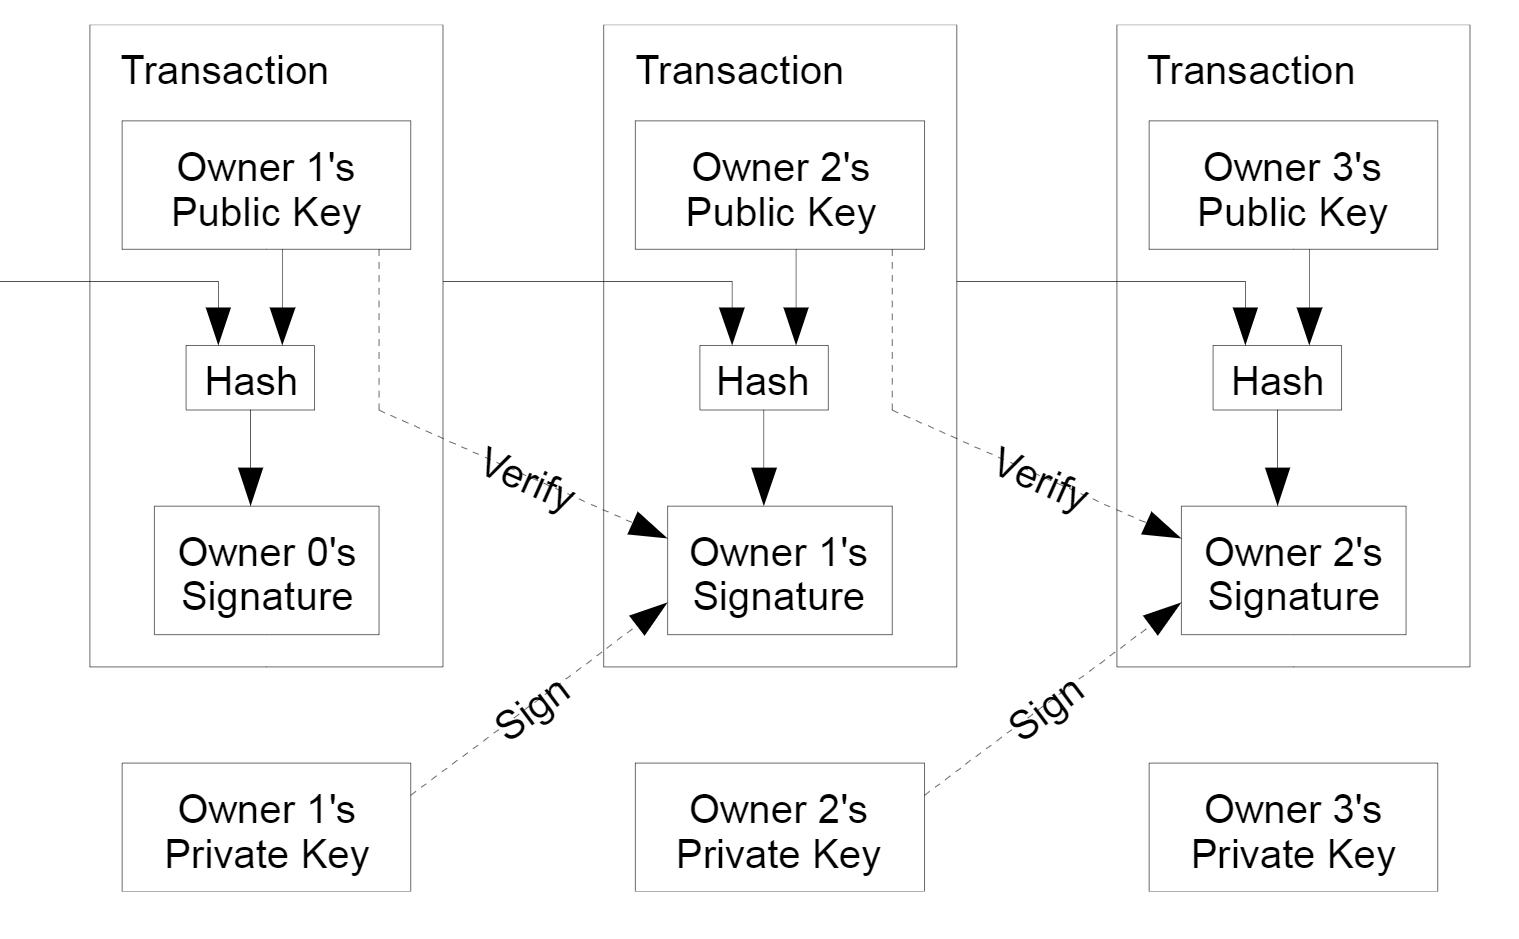
\includegraphics[width=.95\textwidth]{chain-ownership}
    \caption{Chain of ownership for unit of currency. Taken from~\cite{NakamotoBitcoin:System}.}
    \label{fig:chain-ownership}
\end{figure}

\subsubsection{Value}
Besides the system described above, the term `Bitcoin' also refers to a basic \textit{unit} of the currency. Bitcoin is further divisible into smaller units. The smallest unit is 1~Satoshi. 1~Bitcoin contains 100,000,000~Satoshi. 1~Bitcoin at the time of writing has a value of EUR~5~666. The value of Bitcoin is very volatile and has increased and decreased by tens or percents, sometimes even within hours~\cite{Adkisson2018WhyVolatile}. The peak in the value of Bitcoin has occurred on December~16,~2017 when 1 Bitcoin was traded for around USD~19,700~\cite{WolfieZhao2017BitcoinHigh}.

\subsubsection{Incentives}\label{sec:incentives}
A node that manages to successfully mine a block, collects fees from all the included transactions, which poses as an incentive for the nodes to stay honest and keep mining new blocks. In addition to the transaction fees, there is a reward associated with each newly mined block. This reward at the time of writing is 12.5 coins and halves every 210,000 blocks~\cite{Judmayer2017BlocksMechanisms}, with expected decrease again in 2020. The reward is a transaction with no inputs and is the only exception, where the outputs of a transactions are higher than its inputs. The reward for mining a block will decrease to zero approximately in 2140. The supply of the currency is therefore limited and there is an upper bound to the number of Bitcoins that will ever exist\footnotemark.

\footnotetext{As~\cite[p. 38]{Judmayer2017BlocksMechanisms} notes, this limit is only ensured pragmatically and is only valid if majority of the network observes this rule.}

\subsubsection{Altcoins}
The Bitcoin proposal and the first reference client were both published publicly. Not only this allowed for easy adoption within the community, it also enabled creation of cryptocurrencies derived from Bitcoin. These cryptocurrencies, that build on top of Bitcoin and only change few aspects of the system are known as \textit{altcoins}~\cite{Judmayer2017BlocksMechanisms}. Some of these currencies gained exchange value and are still in use by the general public. Others may be targeted on a specific use-case or are only used by narrow communities. Furthermore, some of these altcoins can also serve as proof-of-concept for any improvement proposals for the Bitcoin network~\cite{Tarasiewicz2015ChapterExperiments}. Litecoin, Dogecoin, Namecoin and Talkcoin\footnotemark are only few of the many examples of altcoins. Their differences from Bitcoin and their uses are shown in Table~\ref{tab:altcoins}.
% 
\footnotetext{\url{https://litecoin.org/}\\
\url{https://dogechain.info/}\\
\url{https://namecoin.org/}\\
\url{https://bitcointalk.org/index.php?topic=781207/} all accessed 18-05-2018}
% 
\begin{table}[ht]
    \centering
    \begin{tabularx}{\textwidth}{|l|X|m{10em}|}
         \hline
         \textbf{Name}&\textbf{Main difference from Bitcoin}&\textbf{Use}\\
         \hline
         \hline
         Litecoin&Shorter block time, different \acrshort{pow} algorithm&Value exchange\\
         \hline
         Dogecoin&Shorter block time&Humorous\\
         \hline
         Namecoin&Possible distributed data storage&Domain name registration (.bit), various other uses\\
         \hline
         Talkcoin&Possible message exchange between users, faster block time&Chatting\\
         \hline 
    \end{tabularx}
    \caption{Comparison of selected altcoins.}
    \label{tab:altcoins}
\end{table}
% 
\subsection{Ethereum}

Ethereum is a decentralised computing platform, that runs small programs called \textit{smart contracts}. It builds on similar concepts as Bitcoin, such as blockchain and consensus based on proof-of-work. Smart contracts are written in Ethereum Virtual Machine bytecode and executed by the \acrfull{evm}. Ethereum was proposed in 2013 by a cryptocurrency researcher Vitalik Buterin and was launched in an \acrlong{ico}\footnotemark  in 2014. 
% 
\footnotetext{In an \acrfull{ico} a small percentage of cryptocurrency is sold to a small percentage of backers in a capital-raising process. \url{https://www.investopedia.com/terms/i/initial-coin-offering-ico.asp}, accessed 10-04-2018}
% 
It is currently developed by a Swiss non-profit organisation \textit{Ethereum Foundation}.\footnotemark
% 
\footnotetext{\url{https://www.ethereum.org/foundation}, accessed 10-04-2018}

\subsubsection{Principle of operation}
While in Bitcoin the blockchain only keeps track of unspent transaction outputs, Ethereum blockchain is more complex. It does involve transactions of own currency, which is called \textit{Ether}, but it goes further and introduces other functionality. It is better described as ``\textit{a state machine, where the distributed nodes maintain a shared view of a global state}''~\cite{Tikhomirov2018Ethereum:Perspectives}. Ethereum users issue transactions, which are distributed among the nodes and which change the state of said state machine. Users can make transactions for one of the following reasons~\cite{Atzei2017ASoK}:
\begin{itemize}[noitemsep]
    \item Create a smart contract.
    \item Invoke a function of a smart contract.
    \item Transfer Ether to a smart contract or to another user.
\end{itemize}

Since \acrshort{evm} bytecode is a Turing complete language~\cite{Tikhomirov2018Ethereum:Perspectives, Atzei2017ASoK, Dannen2017IntroducingSolidity}, smart contracts could possibly perform wide variety of computations. However, this has limited use in practice. Every time a transaction invokes a smart contract function, all nodes that observed this transaction, will run the function of the smart contract at once. This redundancy is a desired feature of a decentralised computing platform, such as Ethereum~\cite{EthereumCommunityEthereumDocumentation}, but could lead to a lot of wasted resources, if large quantities of useless computations are to be performed on many nodes at the same time.

To prevent \acrfull{dos} attacks caused by smart contracts, which contain endless loops or very intense computations, there is a price associated with every atomic instruction, which in Ethereum terminology is called \textit{gas}. When a transaction is made, it must specify the maximum amount of gas that can be used to compute the code of a smart contract. If the code of the smart contract includes many computations, the contract will use more gas. If it does not finish computing before it reaches the maximum amount of gas, any changes made by the computations will be reverted, but the gas will not be returned.

To prevent this from happening, users could set the maximum gas limit high enough, so that the smart contract would not run out of gas during its operation. However, to avoid all the participating nodes carrying out huge amount of (potentially useless) computations, the gas is not free and needs to be purchased\footnotemark. 
% 
\footnotetext{The term \textit{gas} was not chosen coincidentally. It is supposed to resemble the gas we put in our cars. The metaphor is as follows: \textit{Our smart contract is the car and the computations performed by the smart contract is the distance driven. If we want to drive further, the car will use more gas. We pay some price per litre of gas, when we stop at the gas station. If we want to drive further, we need to purchase more gas.}}

The gas is purchased at the time when a transaction is made and its price is determined by the free market~\cite{EthereumCommunityEthereumDocumentation}. If an attacker was to invoke an endless loop in a smart contract, the loop would only execute while having enough gas to do so. To spam the network with computationally intense transactions, an attacker would need to purchase high amount of gas and the attack would become too expensive~\cite[p.5]{Atzei2017ASoK}.

\subsubsection{Proof of work}
Similarly as Bitcoin, Ethereum uses proof-of-work to reach consensus. Nodes verify incoming transactions and include them together in a block. This block is then hashed using Ethash, a memory-intensive hash function~\cite[p. 211]{Tikhomirov2018Ethereum:Perspectives}. The hash of the block needs to be below target value to be considered valid. Similarly as in Bitcoin, this process is called mining.  A memory intensive hash function was chosen to target \acrshort{gpu} as the main mining hardware, in order to avoid high barriers for entry. Since \acrshort{gpu} market segment is mainly targeted at other areas, such as gaming or high-performance computing, powerful hardware is already available at the market\footnotemark. The target value for the block hash is adjusted regularly to keep average block production speed constant~\cite{Tikhomirov2018Ethereum:Perspectives}.
% 
\footnotetext{In Bitcoin and other currencies, specialised mining hardware, also referred to as \acrfull{asic} is mainly used for Bitcoin mining. The cost of such hardware and economies of scale make it difficult for small miners to enter the market, therefore weakening one of the main advantages of Bitcoin -- decentralisation~\cite{Tikhomirov2018Ethereum:Perspectives}.}

\subsubsection{Transactions and accounts}
There are two types of accounts defined in Ethereum:
\begin{itemize}[noitemsep]
    \item \textit{\acrfull{eoa}}. \acrshort{eoa}s are accounts controlled by a public-private key-pair that have a non-zero Ether balance. \acrshort{eoa}s can send transactions.~\cite{EthereumCommunityEthereumDocumentation}
    \item \textit{Contract account}. Contract account is an account that has code associated with it. It can run its code and maintain its internal state. It can communicate with other contracts by sending objects called \textit{messages}. Execution of contract's code is triggered by an incoming transaction or a message~\cite{EthereumCommunityEthereumDocumentation}.
\end{itemize}

\subsubsection{Smart contracts}
\acrshort{evm} bytecode is a low-level language, which natively supports cryptographic primitives~\cite{Tikhomirov2018Ethereum:Perspectives}. Smart contracts are usually written in a high-level language and are compiled into \acrshort{evm} bytecode before deployment. The most popular language for writing smart contracts is Solidity, which offers JavaScript-like syntax. Solidity compilers exist for various platforms, including a web-based \acrshort{ide}.

Smart contracts usually cannot perform very extensive calculations, as the \acrshort{evm} is not powerful enough and there is a cost associated with all computations performed by the smart contract. Because of this, every smart contract is either used for some sort of financial transaction or at least requires some funds to be transferred to it, so its code can execute. However, smart contract only exists within the realm of the Ethereum blockchain~\cite{JohnWeldon2016BuildingContract}. It can not fetch data from other sources, nor it can directly interact with the user. This is what \textit{decentralised applications}, or DApps cover. A decentralised application its an application, that runs in a decentralised manner (on the blockchain) and uses smart contracts as part of its logic~\cite[p. 149]{Dannen2017IntroducingSolidity}. On top of the smart contracts, a DApp also contains a regular HTML/CSS/JavaScript front end interface. Such interfaces of DApps are known as Web3 and are considered by many~\cite{Dannen2017IntroducingSolidity, LukeHedger2017CrossingDevelopment} as the third generation of the Web (the first generation was the original World Wide Web, that hosted static pages; the second generation was defined by web-hosted applications and services~\cite{Dannen2017IntroducingSolidity}). Specialised software is needed to interact with the smart contracts in a decentralised application, such as the Ethereum browser Mist\footnote{\url{https://github.com/ethereum/mist}, accessed 22-05-2018} or the browser extension Metamask\footnote{\url{https://metamask.io/}, accessed 22-05-2018}. Although majority of the DApps are built on Ethereum, there are also some that operate on their own blockchain, other than Ethereum~\cite{AlyssaHertigWhatCoinDesk}. Figure~\ref{fig:web3} illustrates the concept of Web3 and DApps.

\begin{figure}
    \centering
    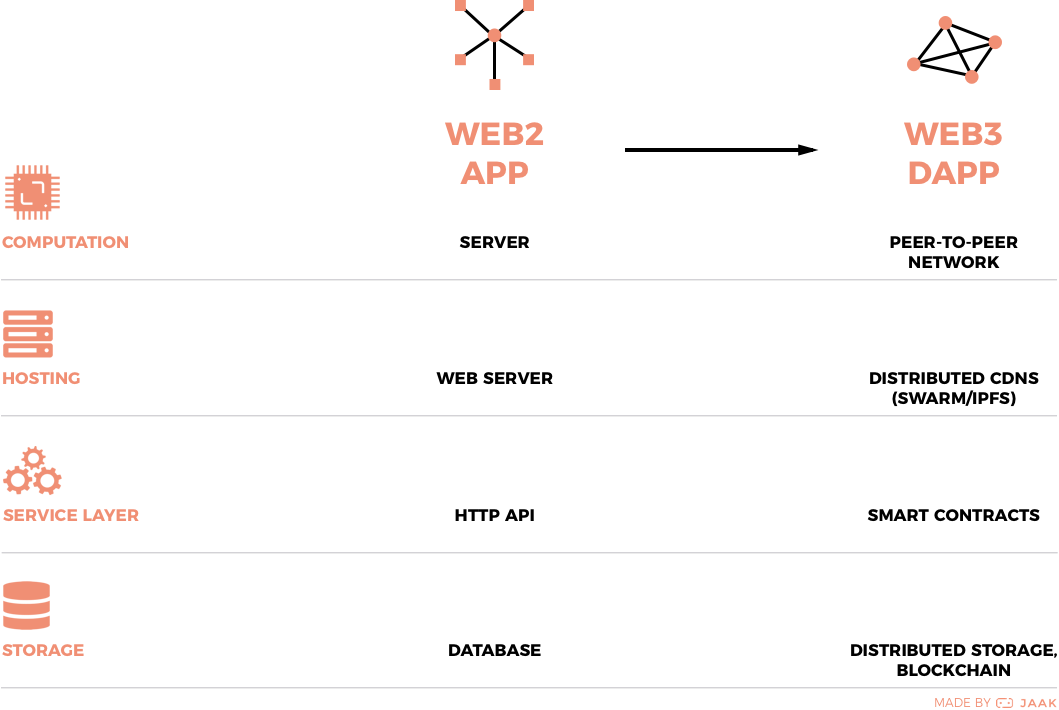
\includegraphics[width=\textwidth]{web3dapp}
    \caption{Comparison of Web2 with Web3. Dicstributed CDNs (Content Delivery Networks), provide hosting to the front end of the DApps (hosting of the HTML/CSS/JavaScript files). Swarm and \acrfull{ipfs} are two exemplary technologies that can provide decentralised such hosting.}
    \label{fig:web3}
\end{figure}


\subsection{Nomenclature}
Despite the existing definitions for words \textit{currency}, \textit{fiat currency} and \textit{cryptocurrency}, there are several naming convention in use today. This paragraph describes, which terms will be used further in this report.

The value of many cryptocurrencies is not backed by any commodity and it depends entirely on the supply/demand relationship. Therefore, by the definition, these cryptocurrencies are also fiat currencies. However, in the literature, the term \emph{fiat currency} is often used when referring to traditional, government issued currencies only. For the rest of this paper we will therefore keep this naming. Regular currencies, such as dollars, euros or crowns will be referred to as fiat currencies.

Virtual, digital money such as Bitcoins, Ether, Litecoin and similar are in some sources named 'coin currencies'. However, in this paper they will be referred to as 'cryptocurrencies' instead, as this is the most common term.
\pagebreak
\section{State of the art}
% 
In recent years, many innovative applications and systems have emerged, that work with Bitcoin, blockchain, smart contracts or other technologies described in previous chapter. We will now explore which of these solutions could be relevant to the idea of a smart contract based currency exchange and we will use these leanings during the development of the system.

\subsection{Network clients //work title}\label{sec:eth-clients}


\subsubsection{Bitcoin}

//WRITE ABOUT BTC CLIENTS

\subsubsection{Ethereum}
% 
To communicate with other peers in the Ethereum network, an Ethereum client is needed. Ethereum client implements the JSON-RPC protocol to talk to its peers

There are three reference Ethereum protocol implementations available:
\begin{enumerate*}[label=(\roman*)]
    \item \textit{Go Ethereum}\footnote{\url{https://geth.ethereum.org/}, accessed 06-05-2018}, written in Go
    \item \textit{Pyethereum}\footnote{\url{https://github.com/ethereum/pyethereum}, accessed 06-05-2018}, written in Python and
    \item \textit{Cppethereum}\footnote{\url{https://github.com/ethereum/cpp-ethereum}, accessed 06-05-2018}, written in C++.
\end{enumerate*}
 and number of competing implementations.
 
\begin{figure}[ht]
    \centering
    \begin{tabular}{|l|c|c|c|l|}
        \hline
        \textbf{Name} & \textbf{\# Watched} & \textbf{\# Starred} & \textbf{\# Forked} & \textbf{Developer}\\
        \hline
        \hline
        go-ethereum & 1779 & 17314 & 5516 & Ethereum Foundation\\
        \hline
        pyethereum & 292 & 2330 & 696 & Ethereum Foundation\\
        \hline
        cpp-ethereum & 529 & 3030 & 1901 & Ethereum Foundation\\
        \hline
        parity & 327 & 4164 & 826 & Parity Technologies\\
        \hline
        ethereumj & 220 & 1505 & 775 & Roman Mandeleil\\ 
        \hline
        ruby-ethereum & 49 & 21 & 37 & Jan Xie\\
        \hline
    \end{tabular}
    \caption{Caption}
    \label{fig:my_label}
\end{figure}
 
The most notable include \textit{Parity}, written in Rust\footnote{\url{https://parity.io/}, accessed 06-05-2018} and ... //Write more
 
 Since all of the mentioned clients are open-source and available on GitHub, we can use these stats to approximately compare their popularity.

As of the time of writing, there are no native Ethereum clients for Android.

//Write more
% 
\subsection{Smart contracts //work title}
% 
//To be written

% 
\subsection{Oracles}
Oraclize
Realitykeys

?something else?

% 
\subsection{Blockchain explorer}
Generally, it is not possible to learn about status of a blockchain (Ethereum, Bitcoin or other) unless we launch a node that directly participates in the blockchain by receiving, verifying and forwarding blocks. However, it is not always feasible to run such a node. If we do not need to deploy any transactions to the network, but only need to receive information from it, we can use a \textit{blockchain explorer}.

A blockchain explorer is a service that participates in the blockchain and exposes its information publicly, so that even parties that are not running a network node can see the information contained in the blockchain\footnotemark. Such information may include transactions, unspent outputs, deployed contracts and other data, usually only visible to participating nodes. 
% 
\footnotetext{At the time of writing, there is no consensus on the use of terms \textit{blockchain explorer} and \textit{block explorer}. Websites offering such services use these terms to market themselves. On the other hand other papers, such as \cite{Kuzuno2017BlockchainBitcoin} use these terms in a different context.}
% 
General cryptocurrency users and services built on top of the blockchain are the most common users of the blockchain explorers\footnotemark/
%
\footnotetext{\url{https://blockchain.info/api}, \url{https://www.blockchain.com/about/index.html}, accessed 12-05-2018}

There are several providers that offer blockchain explorer services. Web interfaces, allowing users to search for and browse transactions and addresses, as well as \acrshort{api}s offering limited number of methods defined by JSON-RPC, are both common practices. Some examples of providers offering these services are \textit{Blockchain}\footnote{\url{https://blockchain.info/}, accessed 12-05-2018}, \textit{Block Explorer}\footnote{\url{https://blockexplorer.com/}, accessed 12-05-2018} and \textit{Block Cypher}\footnote{\url{https://live.blockcypher.com/btc/}, accessed 12-05-2018}. All these examples offer web interface together with an \acrshort{api}.
% 
\pagebreak
\section{System Design}\label{sec:system-design}
% 
//Chapter introduction to be written

There are several possibilities, one wants to exchange cryptocurrency on the internet. Let's consider, that Alice wants to exchange Bitcoin for Ether. She would first find a \acrfull{dcex} that operates with both Bitcoin and Ether. She would probably need to create an account with that exchange and deposit her Bitcoins to that exchange's Bitcoin address. She could then trade the the Bitcoins for the Ether on the exchange's web-page with other registered users. Afterwards, she would withdraw the newly-acquired Ether from her exchange account to her private Ethereum wallet. This is the standard procedure, \textbf{as we learned in the State of the Art. //CHECK THIS} Figure~\ref{fig:arch-ver-exch} shows this standard approach.

\begin{figure}[ht]
    \centering
    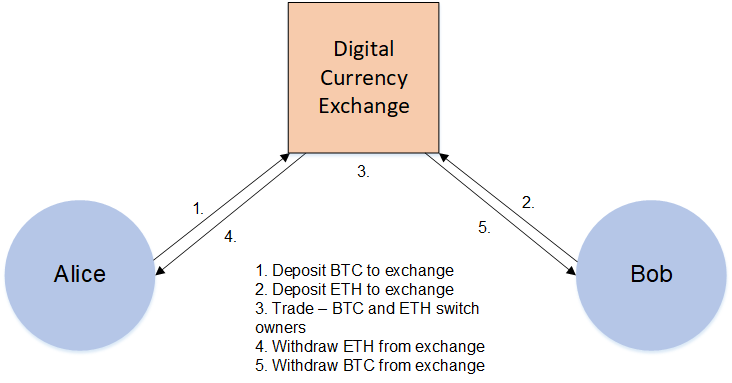
\includegraphics[width=.80\textwidth]{arch-ver-exch}
    \caption{Exchange of currencies using a third party -- a \acrfull{dcex}. The process begins by both Alice and Bobs depositing their respective currencies to the \acrshort{dcex}. \acrshort{dcex} then facilitates the trade of currencies and Alice and Bob can then withdraw their funds from the \acrshort{dcex}.}
    \label{fig:arch-ver-exch}
\end{figure}
% 
\subsection{Architecture}
% 
There are several possibilities, one wants to exchange cryptocurrency on the internet. Let's consider, that Alice wants to exchange Bitcoin for Ether. She would first find a cryptocurrency exchange that operates with both Bitcoin and Ether. She would probably need to create an account with that exchange and deposit her Bitcoins to that exchange's Bitcoin address. She could then trade the the Bitcoins for the Ether on the exchange's web-page with other registered users. Afterwards, she would withdraw the newly-acquired Ether from her exchange account to her private Ethereum wallet. This is more-less the standard procedure, \textbf{as we learned in the State of the Art.}

The issue with this approach is, that Alice needs to fully trust the exchange she chose. Exchange has full control over Alice's funds since she deposited the Bitcoins until she withdraws the Ether. In case that the exchange is attacked by hackers or is not protecting users' funds properly, Alice may never get her money back. The reputation of an exchange may provide little guidance on what exchange is trustworthy, but it is not a definite measure. In the aforementioned case of Mt. Gox, this was the most prominent exchange just weeks before its crash \cite{Popper2014ApparentTimes}.

An alternative approach for Alice could be, that she finds a person who wants to make an opposite trade to hers. Let's further assume, that Bob wants to exchange the same amount of currency from Ether to Bitcoin and that Alice can communicate with Bob by means other than the blockchains or cryptocurrency exchanges (e.g. a cryptocurrency forum). Alice and Bob need to agree on the amounts each of them is going to transfer and they need to exchange their public addresses - namely Alice needs to give Bob her Ethereum public address and Bob needs to give Alice his public Bitcoin address. Alice then sends her Bitcoins to Bob and Bob sends her Ether to Alice. This simple transaction is illustrated in figure \ref{fig:naive-approach}.

\begin{figure}[ht]
    \centering
    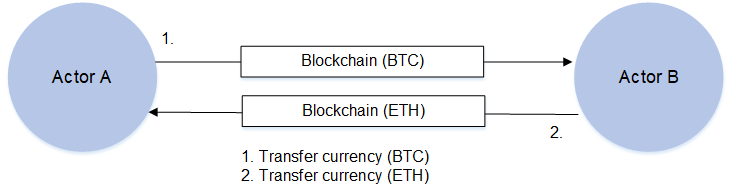
\includegraphics[width=.80\textwidth]{naive-approach}
    \caption{The naive approach to cryptocurrency exchange. Actor A (Alice) wants to buy Bitcoin (BTC) and Actor B (Bob) wants to buy Ether. }
    \label{fig:naive-approach}
\end{figure}

This removes the need to involve a third party in the transaction, but it does not completely solve the problem of trust. Since Alice and Bob might be located in different locations, it may be very difficult if not impossible, to ensure that the other party carries out the transaction as agreed. If Alice sends the funds to Bob, but Bob does not keep his side of the agreement and does not send his funds to Alice, it would be impossible for her to reverse the transaction. 

In an attempt to ensure that both keep their agreement, Alice and Bob could synchronise the moment when they send their transactions to the network. However, this does also not provide a fail-proof solution. For instance, Bob could subsequently send another transaction (transferring his funds to himself) from the same address, which could be processed by the network first, thus rendering the original transaction invalid.

\paragraph{Identification} 
If Alice did not receive the funds as agreed, she might want to involve traditional law-enforcement methods. But since the agreement happened over the internet, it may not be possible to successfully identify Bob.

When an reliable identification of an institution (such as an e-shop) is needed, the concept of public-key certificates has proven useful. The institution engages with a trusted third party, which then verifies the identity of this institution. Afterwards, the third party issues a certificate, that proves the identity of the institution to the visitors from the web, usually for a limited period of time \cite{Lee2013SecurityArchitects}. 

However, for a peer-to-peer relationship, digital certificates do not seem feasible, because the process of verification of someone's identity in real world is a lengthy process. We can now see the emerging need for a system, which does not require trusting a third party, nor trusting the trading partner. A decentralised system running on a blockchain might be the solution to this problem.

\paragraph{Black box architecture}
Let us introduce a `black box' between Alice and Bob. This box could hold funds from both parties and only release them under condition, that both Alice and Bob sent their respective amount. If one of them tried to cheat, the box would not release the funds further. The black box architecture is illustrated in figure \ref{fig:arch-ver0}.
% 
\begin{figure}[ht]
    \centering
    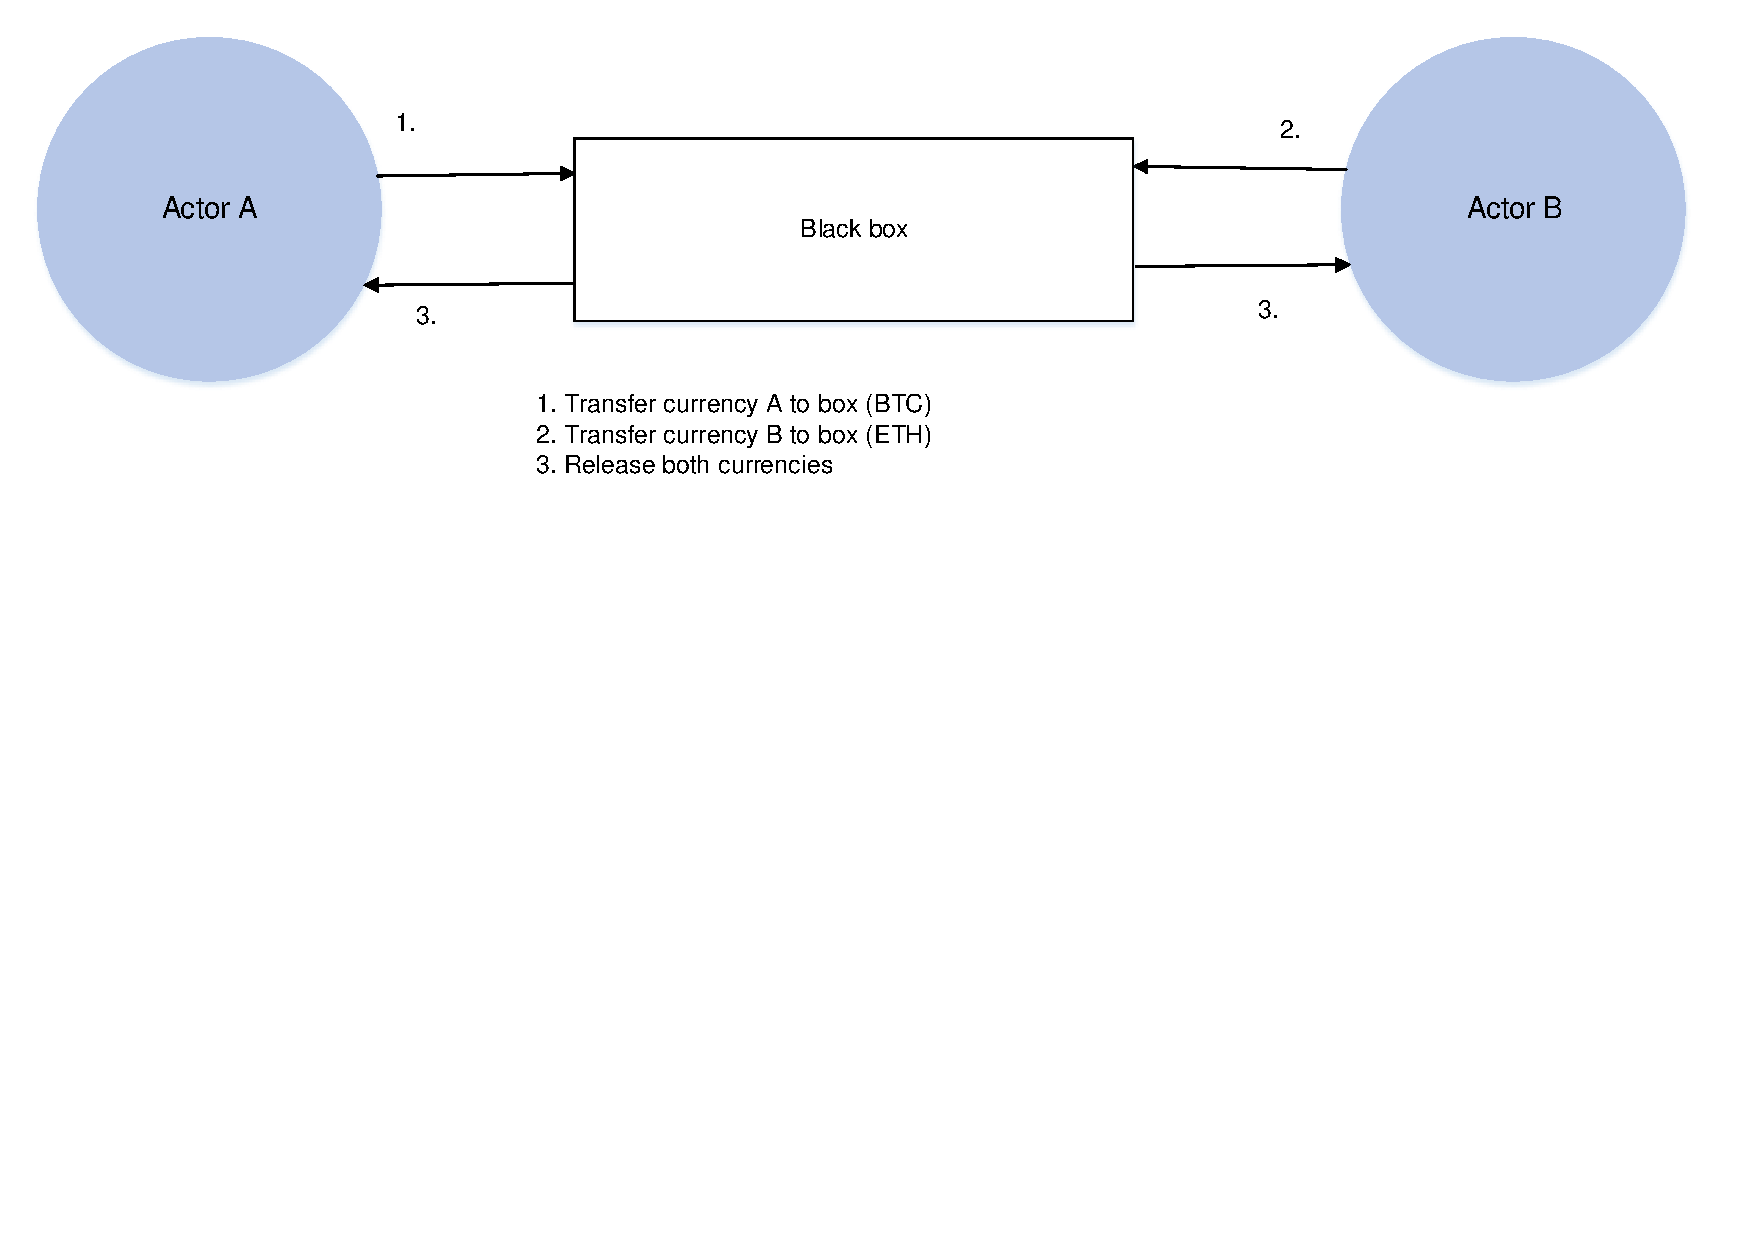
\includegraphics[width=.80\textwidth]{arch-ver0}
    \caption{Black box architecture. The black box spans both blockchains and only releases the funds, if it received the full amount from both parties.}
    \label{fig:arch-ver0}
\end{figure}

The black box is not a third party, rather an automated system that only operates with simple internal logic. This logic should be verifiable by anyone, however, it should not be possible to manipulate this logic by any of the parties. The black box would operate on top of both blockchains and would be decentralised. It would therefore fulfil our requirement for operation without a third party and without requiring the trading parties to trust each other.

This is a plausible architecture for a proposed system. It may be implemented on networks, that enable this kind of transaction control, either via multi-signature wallets (for example Bitcoin) or smart contracts (for example Ethereum). Another advantage is, that the parties now do not need to trust one another. In case of one party tries to cheat, the black box would not release the funds further.

The drawback of this architecture lies in technical complexity. The black box would need to operate on top of \textit{both} blockchains and would require coordination between two networks. The architecture could be simplified in order to remove the need to operate on two blockchains.

\paragraph{Black half-box architecture}
We can achieve similar functionality by only limiting the transaction control to one blockchain. This architecture could be referred to as `black half-box' and is illustrated in figure \ref{fig:half-box-arch}. In this scenario, after initial agreement has been made, Alice proceeds to send funds to the black half-box. This transaction is public and can be verified by Bob. When Bob sees, that the funds are deposited in the box, he can now transfer his funds to Alice. The black half-box queries the blockchain for Bob's transaction in regular intervals. Once the transaction has been successfully included in the blockchain, the black half-box recognises this and can now release Alice's funds to Bob.
% 
\begin{figure}[ht]
    \centering
    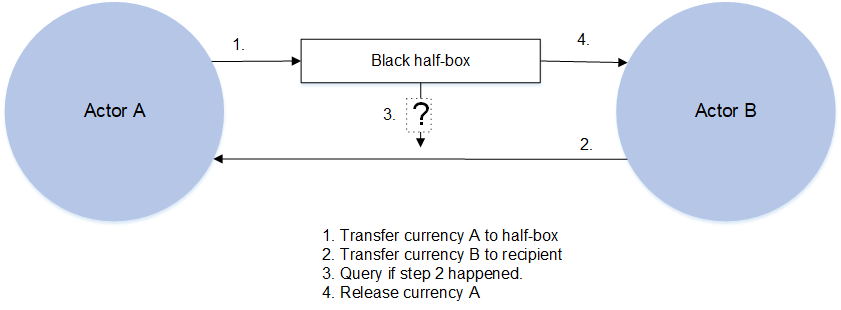
\includegraphics[width=.80\textwidth]{half-box-arch}
    \caption{Black half-box architecture. The box only controls funds on one of the blockchains. The transaction on the other blockchain happens normally. The box queries the blockchain for this transaction, and only releases the funds once it has been processed.}
    \label{fig:half-box-arch}
\end{figure}

This architecture solves the technical drawbacks of the regular black box. However, it can only work safely, if the sequence of steps is followed. In case the funds from Bob to Alice were sent \textit{before} Alice deposited her part in the half-box, Alice is not bound to keep her part of the agreement.

Currently, this architecture could be implemented in two ways: utilising multi-signature wallets

//Write about multi-sig wallet possibilities - 1-way-sig, 2-way-sig, 3-way-sig

//Write about use with Smart contacts, then present the tech-version of the diagram above.






% Regular transactions made in the Bitcoin, Ethereum, Litecoin or other coins are irreversible and once they are processed by the network, they cannot be changed. But what if a condition could be included in the transaction? A `black box' that collects funds 


% that only Some systems (Bitcoin, Ethereum) provide a functionality known as multi-signature wallets



\begin{figure}[ht]
    \centering
    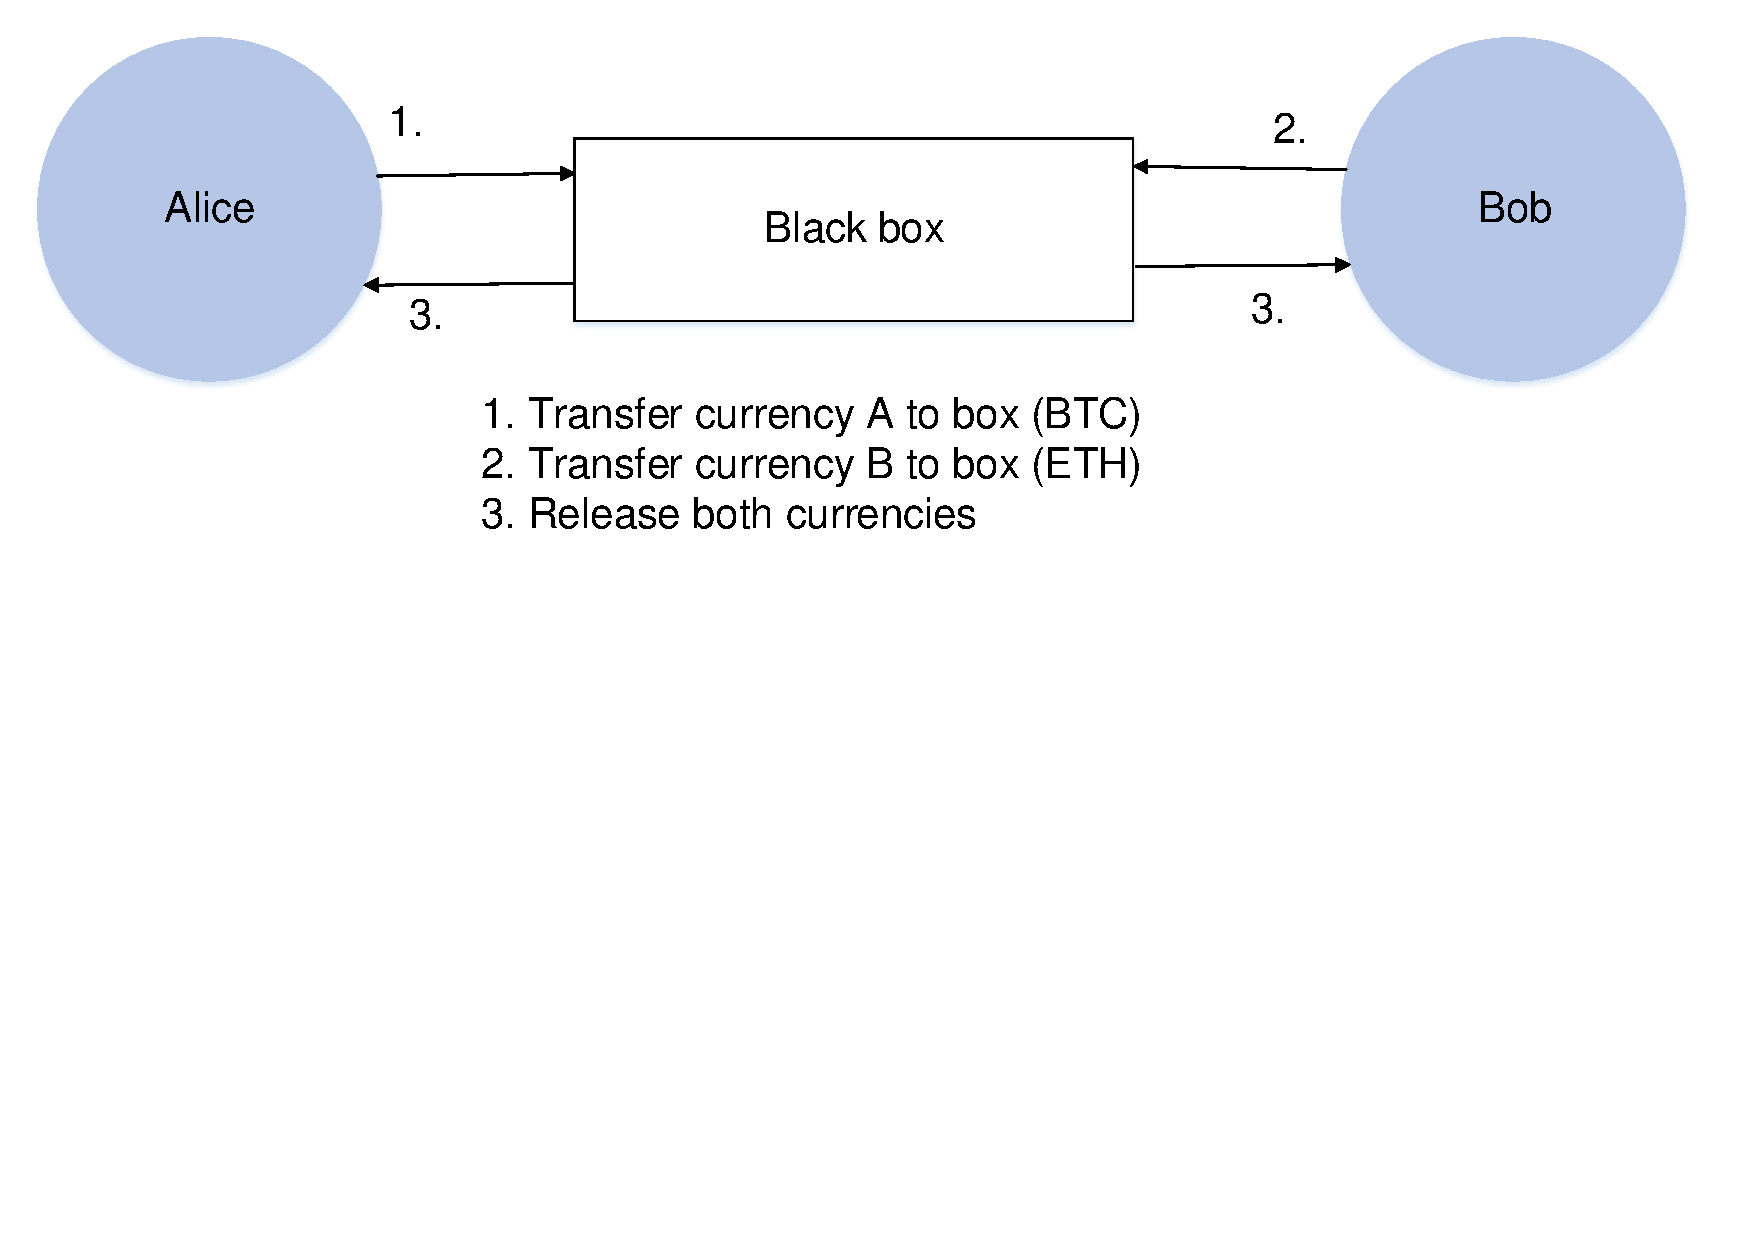
\includegraphics[width=.80\textwidth]{arch-ver1}
    \caption{}
    \label{fig:arch-ver1}
\end{figure}

\subsection{Conclusion}

We can conclude that a system that allows exchange of cryptocurrencies directly between two parties has an elevated degree of complexity. The lack of trust in the virtual currency trading poses as a barrier for several more simple solutions that could be used to exchange fiat currencies. After breaking down the high-level overview into more concrete and implementable architecture, we will describe the development of a prototype in the following section.

//Maybe elaborate a little?


\printbibliography[heading=bibintoc]
\pagebreak


\end{document}
